\chapter{Evaluation}\label{ch:evaluation}
Das folgende Kapitel dient dem Vergleich zwischen BloomFilterTree und der bisherigen Organisation der Bloom-Filter in AMBIENCE. Abschnitt \ref{sec:datensatz} beschreibt den Datensatz, der für die Evaluation verwendet wurde. Er stammt nicht aus AMBIENCE, sondern die Bloom-Filter wurden wie in Abschnitt \ref{sec:aufbau} beschrieben selbst implementiert. Der Versuchsaufbau, d.h. welche Aspekte untersucht und verglichen wurden, findet sich in Abschnitt \ref{sec:versuchsaufbau}. Die erzielten Ergebnisse werden in Abschnitt \ref{sec:ergebnisse} vorgestellt und in Abschnitt \ref{sec:interpretation} ausgewertet.
\section{Datensatz}\label{sec:datensatz}
Obgleich nicht mit echten AMBIENCE-Daten gearbeitet wurde, wurde versucht ein möglichst realistisches Szenario zu erstellen. Folgende Parameter wurden verwendet:
\begin{center}
\begin{table}[htbp]
{\small
\begin{center}
\begin{tabular}[center]{lcc}
\toprule
\textbf{Filtergröße (\textit{m})} & 256 Bit & 512 Bit\\
\midrule
\textbf{Anzahl Bloom-Filter} & 100 & 100\\
\midrule
\textbf{Anzahl eingefügte Objekte (\textit{n})} & 50 & 50\\
\midrule
\textbf{Anzahl Hashfunktionen (\textit{d})} & 4 & 8\\
\bottomrule
\end{tabular}
\end{center}
} % end of tiny
\caption[Datensatz für den Versuchsaufbau]{Datensatz für den Versuchsaufbau.\label{tab:Datensatz}}
\end{table}
\end{center}
Als Wörterbuch wurde die Unix-Datei \texttt{words} verwendet.\footnote{Sie befindet sich auf Unix- und Unix-ähnlichen Systemen normalerweise unter \texttt{/usr/share/dict/words} oder \texttt{/usr/dict/words}.} Daraus wurden jeweils 50 zufällig gewählte Einträge in die Bloom-Filter eingefügt. Dazu wurden wie in Abschnitt \ref{sec:hashfunktionen} erläutert Murmur-Hashfunktionen verwendet. Wie dort ebenfalls erklärt, wurde die Anzahl der zu verwendenden Hashfunktionen berechnet als 
\[d = \Ceil[\Bigg]{\frac{m}{n} * ln(2)}.\]
\noindent
Der \textit{i+1}-te Hashwert wurde dabei jeweils aus dem \textit{i}-ten Hashwert berechnet wie in Abschnitt \ref{sec:bloom-implementierung} beschrieben. Den Bloom-Filtern wurden zunächst zufällige IDs zugewiesen. Sie wurden jeweils in einen BloomFilterTree und in einen Bloom-Filter-Vektor\footnote{Objekte vom Typ \texttt{std::vector<BloomFilter>}.} eingefügt, der die unsortierte Liste repräsentiert.
\newpage
\section{Versuchsaufbau}\label{sec:versuchsaufbau}
Der Versuchsaufbau vergleicht die Indexstruktur BloomFilterTree mit einer unsortierten Liste von Bloom-Filtern an Hand von ausgewählten Aspekten. Für beide Filtergrößen wurden fünf Experimente durchgeführt:  
\begin{enumerate}
\setlength{\itemsep}{20pt}
	\item Ergebnisqualität
	\item CPU-Zeit 
	\item Speicherbedarf 
	\item Aufbaukosten
	\item Komplexität
\end{enumerate}
\paragraph*{Ergebnisqualität}
Zur Ermittlung der Ergebnisqualität wurde die \textit{k}-nächste-Nachbarn-Suche für $k=1$ und $k=3$ auf dem BloomFilterTree ausgeführt. D.h. es wurden jeweils der nächste und die drei nächsten Nachbarn der Anfragefilter in den BloomFilterTree-Objekten mit Filtergröße 256 Bit und Filtergröße 512 Bit ermittelt. Die erzielten Ergebnisse wurden mit den Sollwerten einer regulären \textit{k}-nächste-Nachbarn-Suche verglichen. 
\paragraph*{CPU-Zeit}
Um möglichst plattformunabhängig zu bleiben, wurde die Implementierung in C++ realisiert. Ausgewählte Codebeispiele finden sich im Anhang \ref{ch:anhang}. Zunächst war überlegt worden, teilweise auf bestehende Bibliotheken für Bloom-Filter und Baumstrukturen zurückzugreifen wie die bekannte \textit{Open Bloom Filter}-Bibliothek von Arash Partow.\footnote{Vgl. \url{https://github.com/ArashPartow/bloom} (17.07.2016) für den Quellcode.} Darauf wurde schließlich aus zwei Gründen verzichtet: Einerseits liegt der Fokus der Arbeit nicht auf der Implementierung von Bloom-Filtern. Andererseits stünde durch die Verwendung bestehender Bibliotheken zu befürchten, dass Messergebnisse durch den Rechnenaufwand für nicht benötigte Operationen oder durch in AMBIENCE nicht vorhandene Optimierungen verfälscht würden. 

Eine Bibliothek für B$^+$-Bäume ist z.B. das \textit{STX B+ Tree package} von Timo Bingmann\footnote{Vgl. \url{https://github.com/bingmann/stx-btree} (17.07.2016) für den Quellcode.}. Wie in Abschnitt \ref{sec:bloom-index} dargestellt, sind keine Varianten von Indexstrukturen bekannt, die sich unverändert für AMBIENCE übernehmen ließen. Auch eine bestehende Bibliothek müsste also stark abgewandelt werden. Gleichzeitig könnten dieselben Verfälschungen auftreten wie bei Verwendung einer Bloom-Filter-Bibliothek. So wurde auch davon abgesehen.

Die Klasse \texttt{BloomFilterTree} enthält alle notwendigen Parameter und Operationen zur Organisation der Bloom-Filter. Ihre Header-Datei ist im Anhang \ref{ch:anhang} abgedruckt. In der Klasse \texttt{BloomFilter} wurden alle Parameter und Operationen auf Bloom-Filtern realisiert, die sich im Laufe der Arbeit als wichtig erwiesen. Ihre Header-Datei findet sich ebenfalls im Anhang \ref{ch:anhang}. Die Funktion \texttt{computeSubsetId()} der Klasse \texttt{BloomFilterLeaf}, die die optimale Teilmengen-ID für einen neu einzufügenden Bloom-Filter berechnet, findet sich ebenfalls im Anhang. Die Berechnung der optimalen Obermengen-ID geschieht analog dazu in der Funktion \texttt{computeSupersetId()}, nur dass dazu die Obermengen des neuen Filters betrachtet werden. Der Quellcode der Funktion \mbox{\texttt{simQueryVec()}} der Klasse \texttt{BloomFilterTree}, mit der eine \textit{k}-nächste-Nachbarn-Suche zu einem Anfragefilter in einem BloomFilterTree durchgeführt wird, ist ebenfalls beispielhaft im Anhang \ref{ch:anhang} abgedruckt.

Zur Messung der CPU-Zeit wurde die C++-Bibliothek \texttt{chrono} verwendet. Es wurden jeweils die Ausführungszeiten der Funktionen \texttt{simQuery()} und \texttt{simQueryVec()} für $k=1$ bzw. $k=3$ ermittelt. Diese implementieren die nächste-Nachbarn-Suche bzw. die \textit{k}-nächste-Nachbarn-Suche wie in Abschnitt \ref{sec:knn}) beschrieben. Die Ausführungszeiten der Funktionen wurden mit den Ausführungszeiten einer regulären \textit{k}-nächste-Nachbarn-Suche verglichen.
\paragraph*{Speicherbedarf} 
Da der BloomFilterTree nur Zeiger auf Bloom-Filter-Objekte enthält und nicht die Datenstrukturen selbst, ist sein Speicherbedarf eher gering. Zur Ermittlung des Speicherbedarfs wurde daher von den tatsächlich allokierten Instanzen der Klasse \texttt{BloomFilter} ausgegangen. Das sind bei einer unsortierten Liste alle eingefügten Bloom-Filter, beim BloomFilterTree zusätzlich die Vereinigungsfilter aller Knoten. Diese Speicherbedarfe wurden für BloomFilterTree und unsortierte Liste ermittelt und gegenüber gestellt. 
\paragraph*{Aufbaukosten}
Als Maß für die Aufbaukosten von BloomFilterTree und unsortierter Liste wurde die Zeitkomplexität des Einfügens aller Elemente verwendet. Diese liegt für Objekte vom Typ \texttt{std::vector} mit \textit{n} Elementen durchschnittlich in $O(1)$ für die verwendete Funktion \texttt{std::vector::push\_back()}.\footnote{Vgl. \url{http://www.cplusplus.com/reference/vector/vector/push_back/} (17.07.2016).}

Beim BloomFilterTree setzt sich die Komplexität der Einfüge-Operation aus der Berechnung der optimalen Teilmengen- und Obermengen-IDs und dem tatsächlichen Einfügen des Objekts zusammen. Wie in Abschnitt \ref{sec:einfügen} dargestellt, ist die Berechnung der Teilmengen-IDs aufwändig und macht die Einfüge-Operation deutlich teurer als das kanonische Einfügen im B$^+$-Baum. Die Operationen mit der größten Zeitkomplexität sind hierbei das Sortieren der freien und "`guten"' IDs. Die Kosten für den Aufbau der Indexstruktur liegen damit insgesamt in $O(n\ast log(n))$ für einen BloomFilterTree mit \textit{n} Elementen. 
\paragraph*{Komplexität}
Zur Ermittlung der Komplexität der unterschiedlichen Suchalgorithmen wurde die Anzahl der Vergleiche, die zur Anfragebeantwortung notwendig sind, als Maß verwendet. Diese wurden für BloomFilterTree und unsortierte Liste ermittelt und verglichen. Für den BloomFilterTree wurden dazu Varianten der Funktionen \texttt{simQuery()} und \texttt{simQueryVec()} implementiert, die die Anzahl an durchgeführten Vergleichen exakt mitprotokollieren.
\newpage
\enlargethispage{2\baselineskip}
\section{Ergebnisse}\label{sec:ergebnisse}
Im Folgenden werden die Ergebnisse der fünf Experimente mit den beschriebenen Parametern vorgestellt. 
\paragraph*{Ergebnisqualität}
Abbildung \ref{fig:quality} stellt die Ergebnisqualität der \textit{k}-nächste-Nachbarn-Su\-che dar. Die Suche wurde jeweils für $k=1$ und $k=3$ auf BloomFilterTree-Objekten mit den Filtergrößen 256 Bit bzw. 512 Bit durchgeführt. Die Teilgrafiken \ref{fig:quality:1} und \ref{fig:quality:2} zeigen die Ergebnisse für $k=1$. Der jeweilige Sollwert für das Ergebnis ist darin grün, der Messwert blau markiert. Stimmen Messwert und Sollwert überein, wurde mit der BloomFilterTree-Variante der \textit{k}-nächste-Nachbarn-Suche ein optimales Ergebnis erzielt. In diesem Fall ist nur die blaue Markierung vorhanden. Der quadratische Fehler von Messwert gegenüber Sollwert ist in Rot angegeben.

Die Teilgrafiken \ref{fig:quality:3} und \ref{fig:quality:4} zeigen die Ergebnisse der \textit{k}-nächsten-Nachbarn-Suche im BloomFilterTree für $k=3$. Die Messwerte sind darin in drei Blaustufen markiert: Der dunkelste Blauton bezeichnet den nächsten Nachbarn, der mittlere Blauton den zweit- und der hellste Blauton den drittnächsten Nachbarn des Anfragefilters im BloomFilterTree. Die Abweichung von den Sollwerten lässt sich am mittleren quadratischen Fehler der Messwerte gegenüber den Sollwerten ablesen. Dieser ist in Rot angegeben. 
\begin{figure}[hpbt]
	\centering
	\captionabove[Ergebnisqualität der \textit{k}-nächste-Nachbarn-Suche]{Ergebnisqualität der \textit{k}-nächste-Nachbarn-Suche.}\label{fig:quality}
	\subfloat[]{
	\label{fig:quality:1}
 	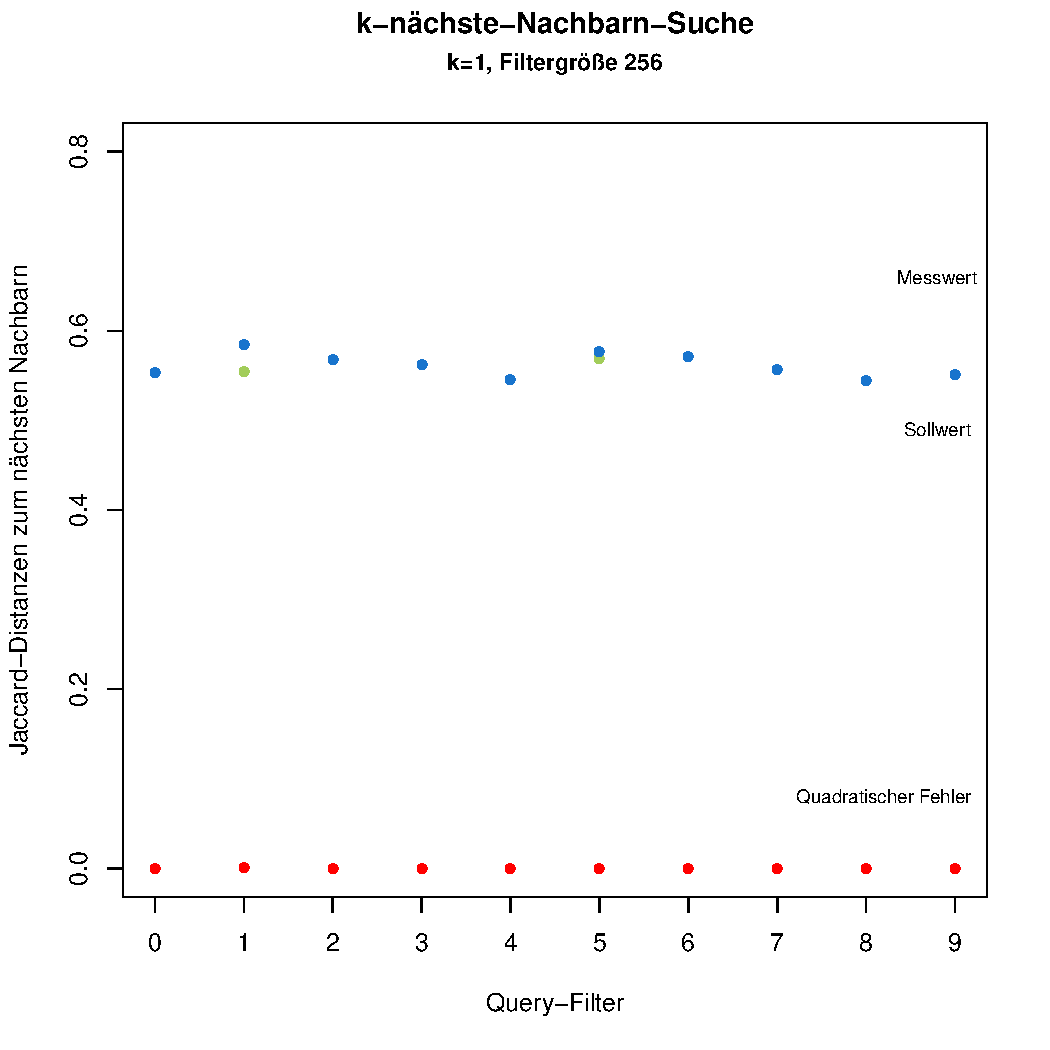
\includegraphics[width=0.48\textwidth]{pictures/nn_256.pdf}}
 	\hspace{0.01\textwidth}
 	\subfloat[]{
 	\label{fig:quality:2}
 	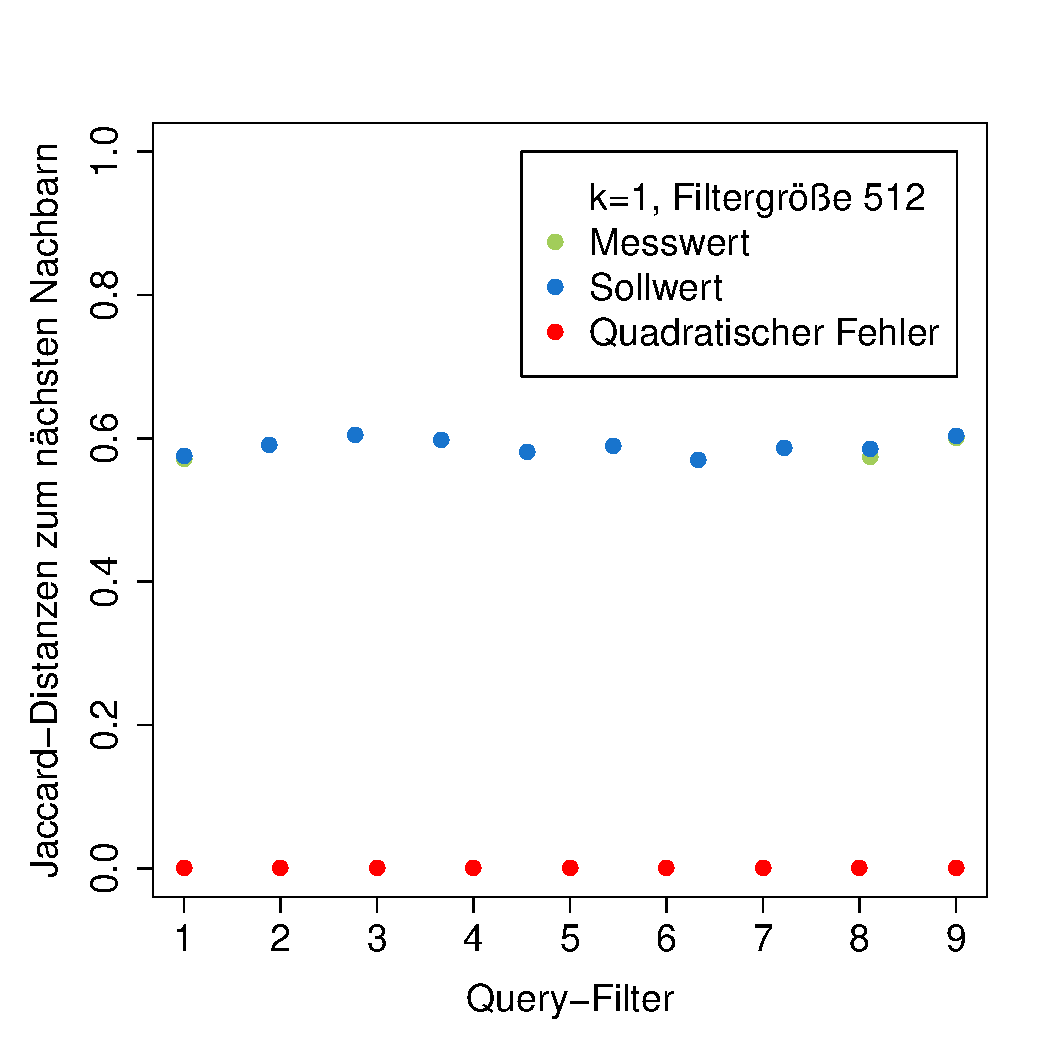
\includegraphics[width=0.48\textwidth]{pictures/nn_512.pdf}}\\[0pt]
 	\subfloat[]{
 	\label{fig:quality:3}
	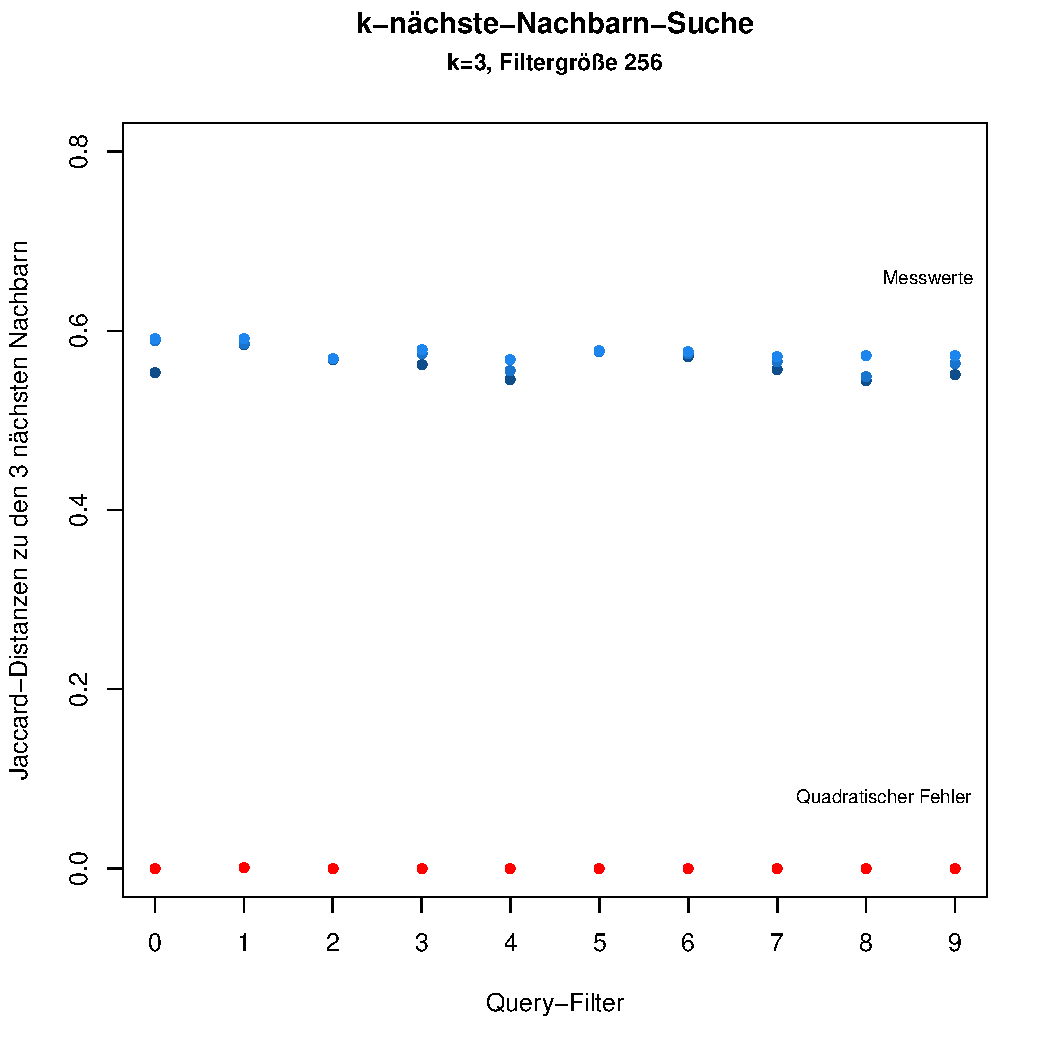
\includegraphics[width=0.48\textwidth]{pictures/nn3_256-2.pdf}}
	\hspace{0.01\textwidth}
	\subfloat[]{
	\label{fig:quality:4}
	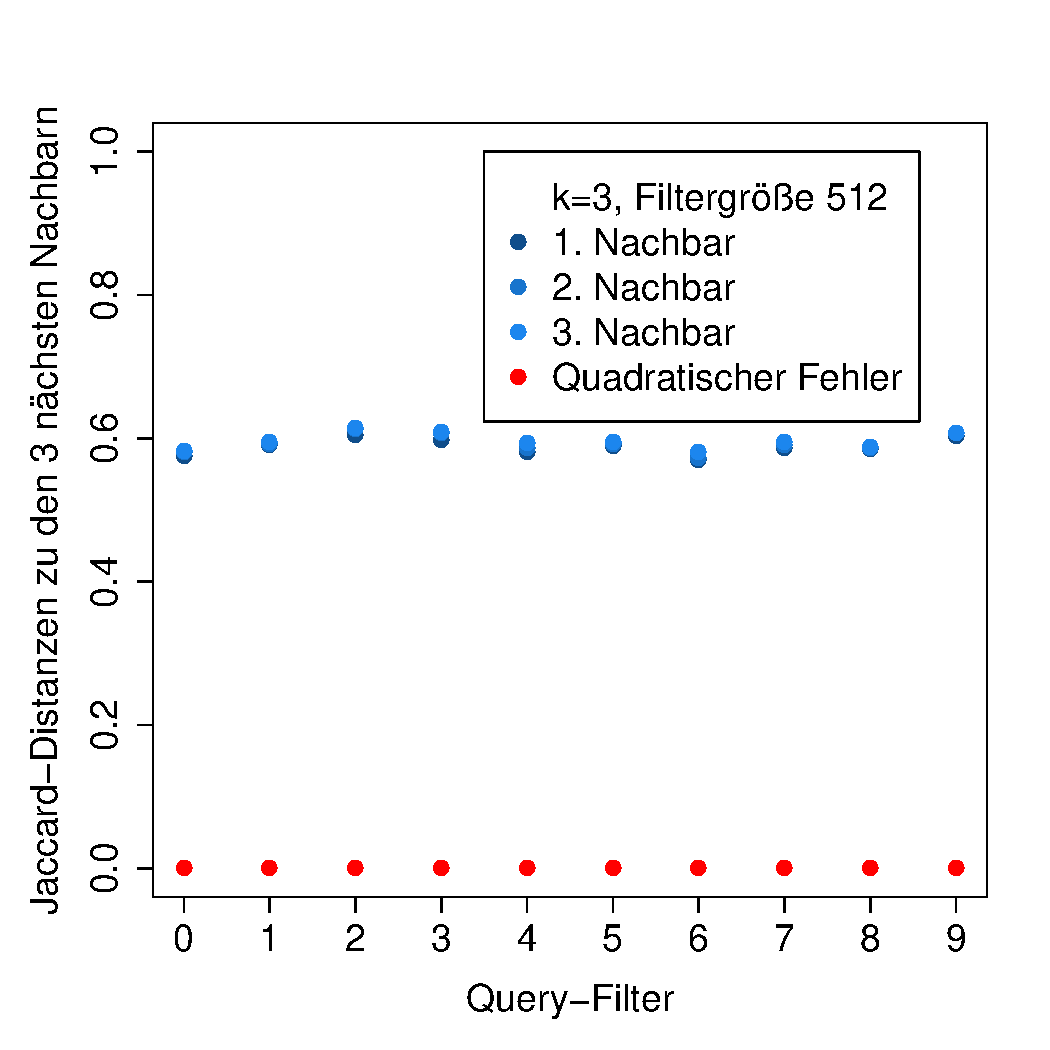
\includegraphics[width=0.48\textwidth]{pictures/nn3_512-2.pdf}}
\end{figure}
\paragraph*{CPU-Zeit} 
Abbildung \ref{fig:cputime} stellt die CPU-Zeit zur Ausführung der \textit{k}-nächste-Nachbarn-Suche dar. Die CPU-Zeit wurde jeweils für $k=1$ und $k=3$ für die Datenstrukturen BloomFilterTree und unsortierte Liste ermittelt. Auch hier wurden jeweils zwei Filtergrößen verwendet, 256 Bit und 512 Bit. Die Teilgrafiken \ref{fig:cputime:1} und \ref{fig:cputime:2} zeigen die Ergebnisse fr $k=1$. Die Teilgrafiken \ref{fig:cputime:3} und \ref{fig:cputime:4} zeigen die Ergebnisse für $k=3$. Die Ergebnisse für den BloomFilterTree sind in Abbildung \ref{fig:cputime} blau, die Ergebnisse für die unsortierte Liste grün markiert. Ein niedrigerer Wert für die CPU-Zeit ist hier offensichtlich wünschenswert. Er bedeutet, dass die Suche beschleunigt wurde und die gewünschten Ergebnisse schneller gefunden wurden. 
\begin{figure}[hptb]
	\centering
	\captionabove[CPU-Zeit für \textit{k}-nächste-Nachbarn-Suche]{CPU-Zeit für \textit{k}-nächste-Nachbarn-Suche.}\label{fig:cputime}
	\subfloat[]{
	\label{fig:cputime:1}
	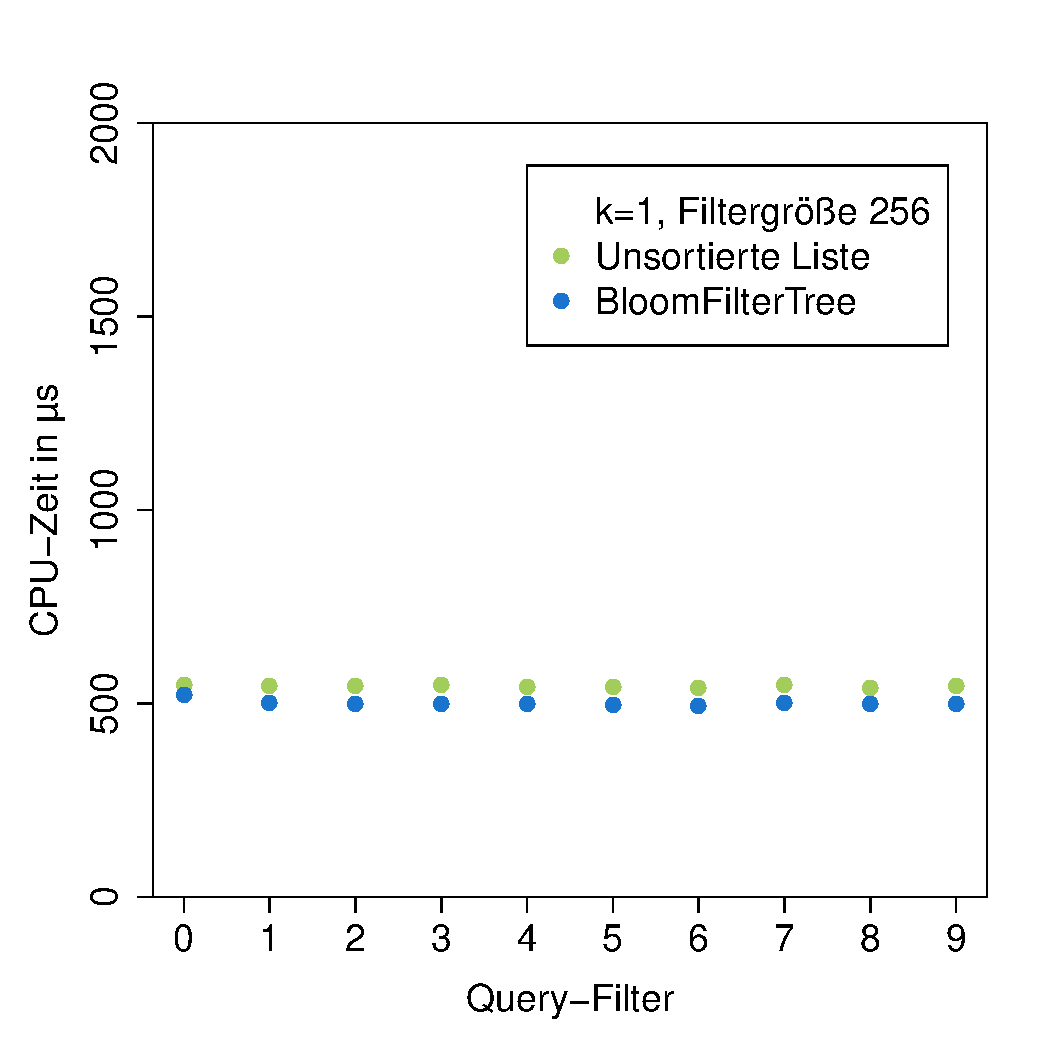
\includegraphics[width=0.48\linewidth]{pictures/cputime_nn_256.pdf}}  
	\hspace{0.01\textwidth}
	\subfloat[]{
	\label{fig:cputime:2}
	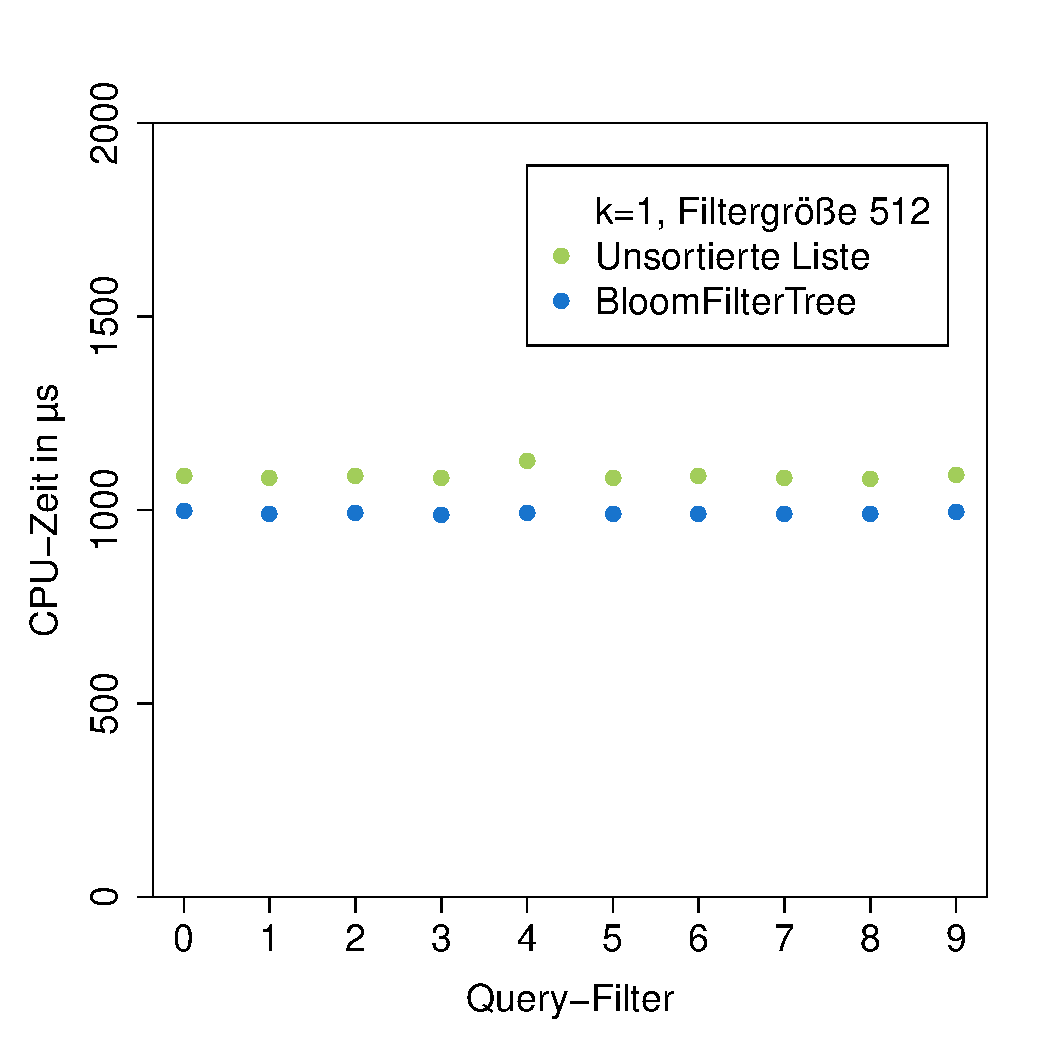
\includegraphics[width=0.48\linewidth]{pictures/cputime_nn_512.pdf}}\\[0pt] % horizontal break
	\subfloat[]{
	\label{fig:cputime:3}
	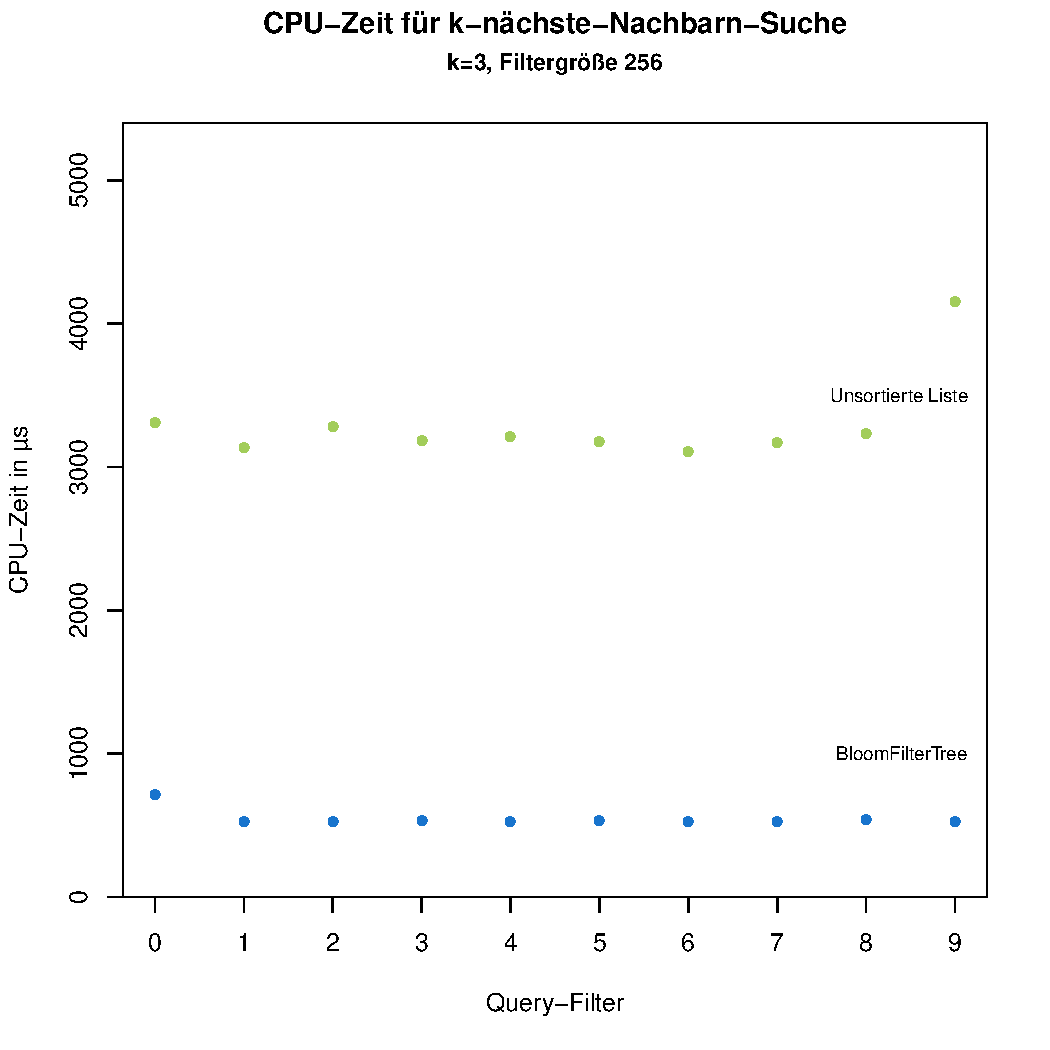
\includegraphics[width=0.48\linewidth]{pictures/cputime_nn3_256.pdf}}
	\hspace{0.01\textwidth}
	\subfloat[]{
	\label{fig:cputime:4}	
	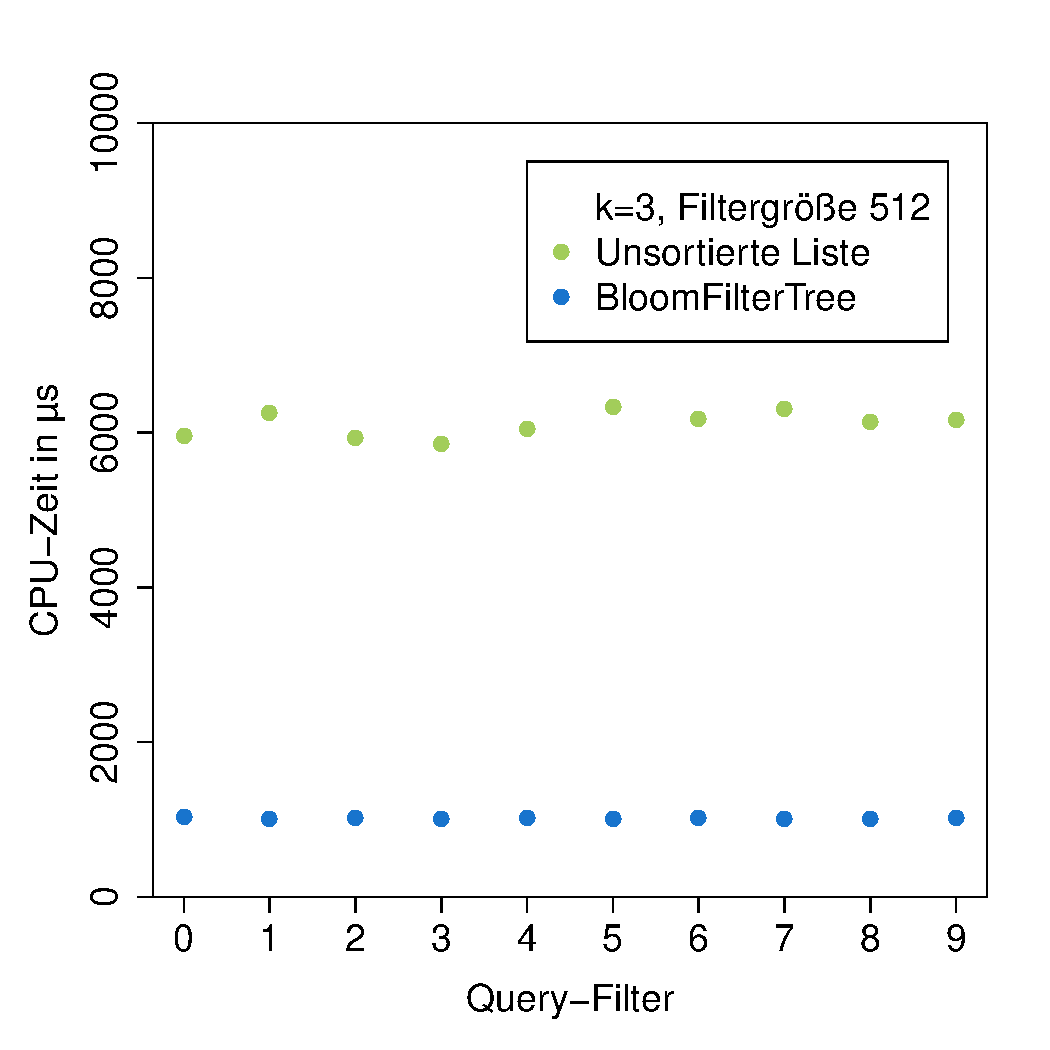
\includegraphics[width=0.48\linewidth]{pictures/cputime_nn3_512.pdf}}
\end{figure}
\paragraph*{Speicherbedarf}
Abbildung \ref{fig:pic18} stellt den Speicherbedarf für BloomFilterTree und unsortierte Liste gegenüber. Objekte vom Typ BloomFilterTree sind darin blau, Objekte vom Typ \texttt{std::vector<BloomFilter>} grün markiert. Ein höherer Wert ist so zu lesen, dass mehr Speicher für die jeweilige Datenstruktur benötigt wird. Das ist also ungünstiger bzw. diese Datenstruktur ist teurer. Für beide Datenstrukturen wurden jeweils Instanzen mit 256 Bit und 512 Bit Filtergröße untersucht. 
\paragraph*{Aufbaukosten}
Abbildung \ref{fig:pic20} stellt die Aufbaukosten der angelegten Objekte dar. Aufbaukosten bedeutet in diesem Zusammenhang: Wie rechenintensiv ist das Einfügen aller Objekte in die Datenstruktur? Im hier verwendeten Versuchsaufbau wurden jeweils 100 Bloom-Filter-Objekte in die Datenstrukturen BloomFilterTree und unsortierte Liste eingefügt. Die Aufbaukosten für Objekte vom Typ \texttt{std::vector<BloomFilter>} sind in Abbildung \ref{fig:pic20} grün markiert. Die Aufbaukosten für Objekte vom Typ BloomFilterTree sind blau markiert. Ein niedriges Ergebnis repräsentiert somit eine einfach zu befüllende Datenstruktur. Das ist tendenziell wünschenswert. 
\begin{figure}[hptb]
	\centering
	\captionabove[Speicherbedarf für Datenstrukturen]{Speicherbedarf für Datenstrukturen.}\label{fig:pic18}
	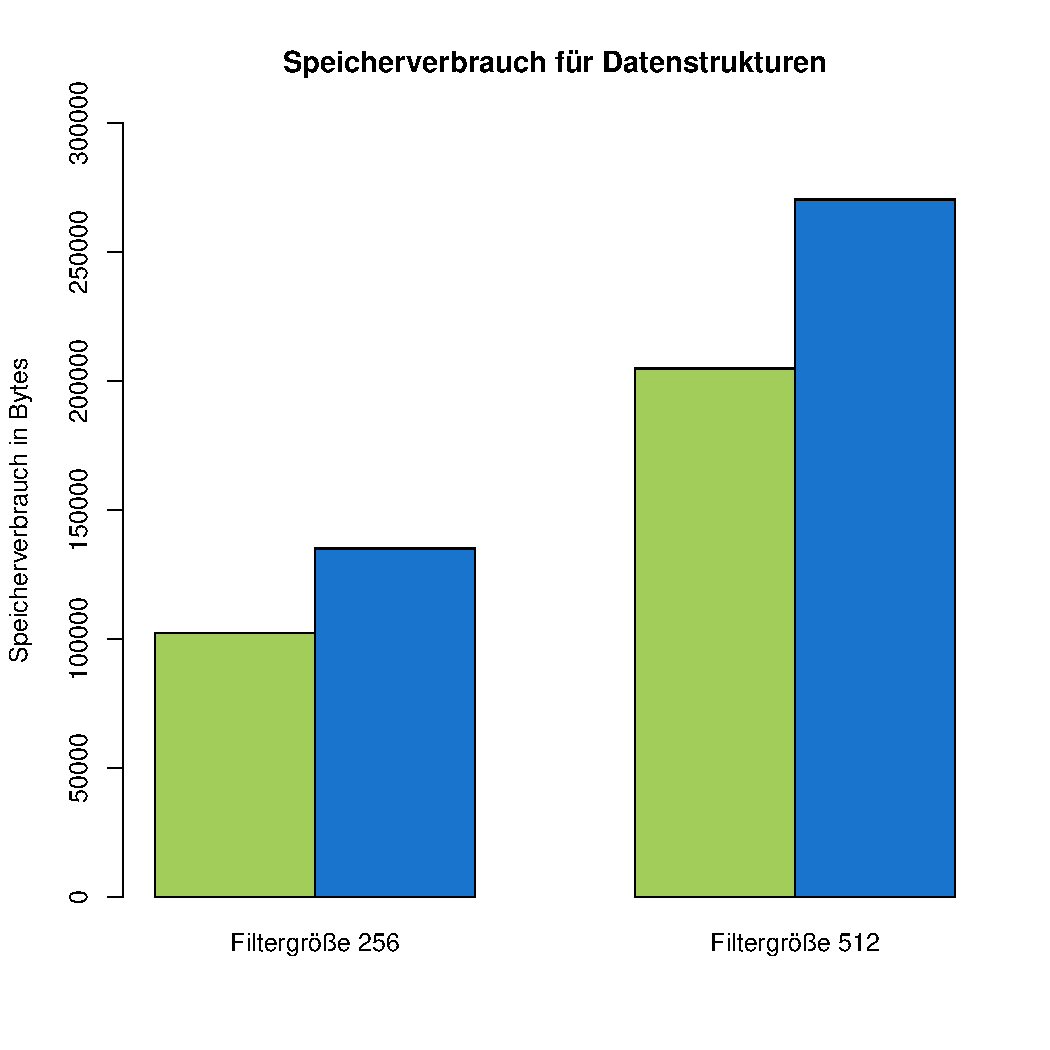
\includegraphics[scale=0.7]{pictures/mem.pdf}\\
	\captionabove[Aufbaukosten für Datenstrukturen]{Aufbaukosten für Datenstrukturen.}\label{fig:pic20}
	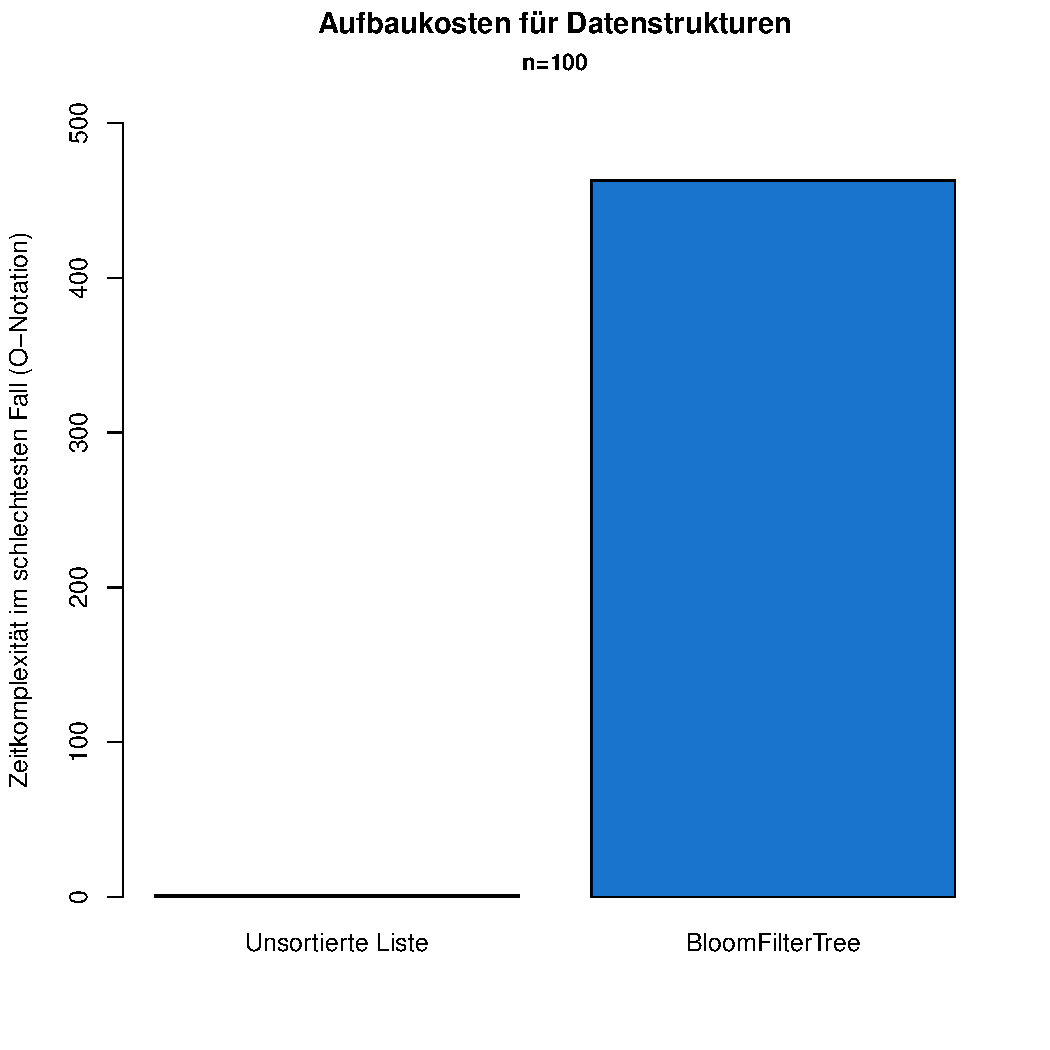
\includegraphics[scale=0.7]{pictures/cost.pdf}
\end{figure} 
\paragraph*{Komplexität}
Abbildung \ref{fig:pic19} stellt die Komplexität der \textit{k}-nächste-Nachbarn-Suche dar. Wie in Abschnitt \ref{sec:versuchsaufbau} beschrieben, wird die Komplexität hierbei als Anzahl von \mbox{Vergleichen} aufgefasst, die Anfragebearbeitung nötig sind. Für die unsortierte Liste wird hierbei die reguläre Implementierung der \textit{k}-nächste-Nachbarn-Suche verwendet, deren Zeitkokmplexität in $O(n^2)$ liegt. Für die Suche im BloomFilterTree wird die in Abschnitt \ref{sec:knn} ausführlich beschriebene, optimierte Variante der eigenen Implementierung verwendet. Die Ergebnisse für die Suche im BloomFilterTree sind in Abbildung \ref{fig:pic19} blau markiert. Die Ergebnisse der unsortierten Liste sind grün markiert.

Ein niedriges Ergebnis ist hier wünschenswert. Das bedeutet, dass die \textit{k}-nächste-Nach\-barn-Suche auch theoretisch, d.h. unabhängig von der verwendeten Maschine, optimiert und beschleunigt werden konnte. Die Zeitersparnis ist somit nicht nur an Hand der reduzierten CPU-Zeiten, sondern auch durch die reduzierte Komplexität ersichtlich. 
\begin{figure}[hptb]
	\centering
	\captionabove[Komplexität der \textit{k}-nächste-Nachbarn-Suche]{Komplexität der \textit{k}-nächste-Nachbarn-Suche.}\label{fig:pic19}
	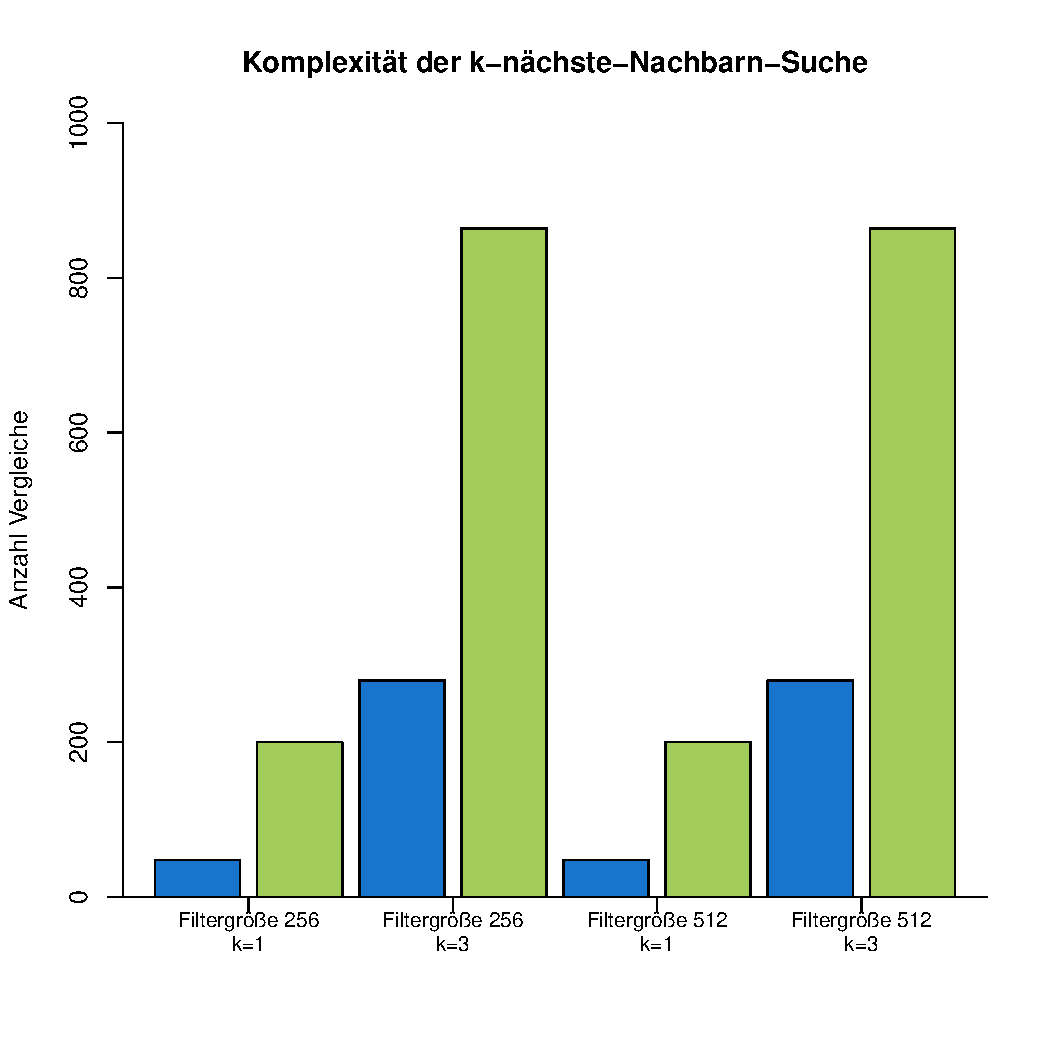
\includegraphics[scale=0.7]{pictures/compl.pdf}
\end{figure}
\newpage
\section{Interpretation}\label{sec:interpretation}
Wie in Abschnitt \ref{sec:datensatz} dargestellt, wurde die Evaluation mit zehn Anfragefiltern pro Experiment durchgeführt. Die Ergebnisse sind also dazu geeignet, etwaige Ausreißer zu erkennen, wenn z.B. ein Ergebnis unverhältnismäßg stark von den durchschnittlich erzielten Werten abweicht. Das gilt insbesondere für die Ergebnisse der CPU-Zeitmessung, die in der Regel wegen schwankender Nutzlast der verwendeten Maschine und nicht exakt vorhersehbaren CPU-Schedulings gewissen Schwankungen unterliegen. Demnach kann hierbei das Minimum der erzielten Messwerte als Benchmark angesehen werden. 
\paragraph*{Ergebnisqualität}
Die Ergebnisse der \textit{k}-nächste-Nachbarn-Suche mit $k=1$ stimmen zum größten Teil mit den Sollwerten überein. Lediglich beim BloomFilterTree mit 256 Bit-Bloom-Filtern treten zwei abweichende Ergebnisse auf (vgl. Abbildung \ref{fig:quality:1}). Bei der \textit{k}-nächste-Nachbarn-Suche mit $k=3$ und 256-Bit-Filtern treten bei 30 Ergebnissen fünf abweichende Einzelergebnisse auf (vgl. Abbildung \ref{fig:quality:3}). Im BloomFilterTree mit 512-Bit-Filtern treten dabei von 30 Ergebnissen sechs abweichende Einzelergebnisse auf (vgl. Abbildung \ref{fig:quality:4}). 

Der quadratische Fehler für diese abweichenden Fälle beträgt dabei für $k=1$ und 256 Bit-Bloom-Filter maximal 0.0008548022. Andernfalls beträgt der quadratische Fehler 0. Für $k=3$ und 256 Bit-Bloom-Filter beträgt der mittlere quadratische Fehler bei abweichenden Messwerten maximal 0.0002956207, andernfalls 0. Für $k=3$ und 512 Bit-Bloom-Filter beträgt der mittlere quadratische Fehler maximal 0.00008640455, andernfalls 0.

Das bedeutet: \textit{k}-nächste-Nachbarn-Anfragen werden mit dem entwickelten Verfahren in den meisten Fällen korrekt beantwortet. In wenigen Fällen werden suboptimale Antworten zurückgegeben. Diese sind dennoch als zufriedenstellende Antworten bezüglich des verwendeten Datensatzes und des quadratischen Fehlers zu bezeichnen. Dieses Resultat ist essentiell für die Bewertung des entwickelten Verfahrens. Es kann nur dann zuverlässig eingesetzt werden, wenn es in einem Großteil der Fälle zufriedenstellende Ergebnisse bzw. optimale Antworten liefert. 
\paragraph*{CPU-Zeit}
Die drastisch reduzierte CPU-Zeit ist als entscheidender Vorteil des entwickelten Verfahrens zu betrachten. In der verwendeten Versuchsanordnung kommt sie vor allem bei der \textit{k}-nächste-Nachbarn-Suche mit $k=3$ zum Tragen. Abbildung \ref{fig:zeitersparnis} stellt die jeweils erreichte Zeitersparnis gegenüber. Die grün markierten Werte bezeichnen hierbei die CPU-Zeit für die \textit{k}-nächste-Nachbarn-Suche in Prozent gegenüber einer unsortierten Liste.  Die Ergebnisse für $k=1$ und 256 Bit- bzw. 512 Bit-Bloom-Filter sind in den Teilgrafiken \ref{fig:zeitersparnis:1} und \ref{fig:zeitersparnis:2} dargestellt. Die Ergebnisse für $k=3$ und 256 Bit- bzw. 512 Bit-Bloom-Filter sind in den Teilgrafiken \ref{fig:zeitersparnis:3} und \ref{fig:zeitersparnis:4} zu sehen. 
\begin{figure}[hpbt]
	\centering
	\captionabove[\mbox{CPU-Zeitersparnis für \textit{k}-nächste-Nachbarn-Suche im BloomFilterTree}]{CPU-Zeitersparnis für \textit{k}-nächste-Nachbarn-Suche im Bloom-Filter-Tree.}\label{fig:zeitersparnis}
	\subfloat[]{
	\label{fig:zeitersparnis:1}
	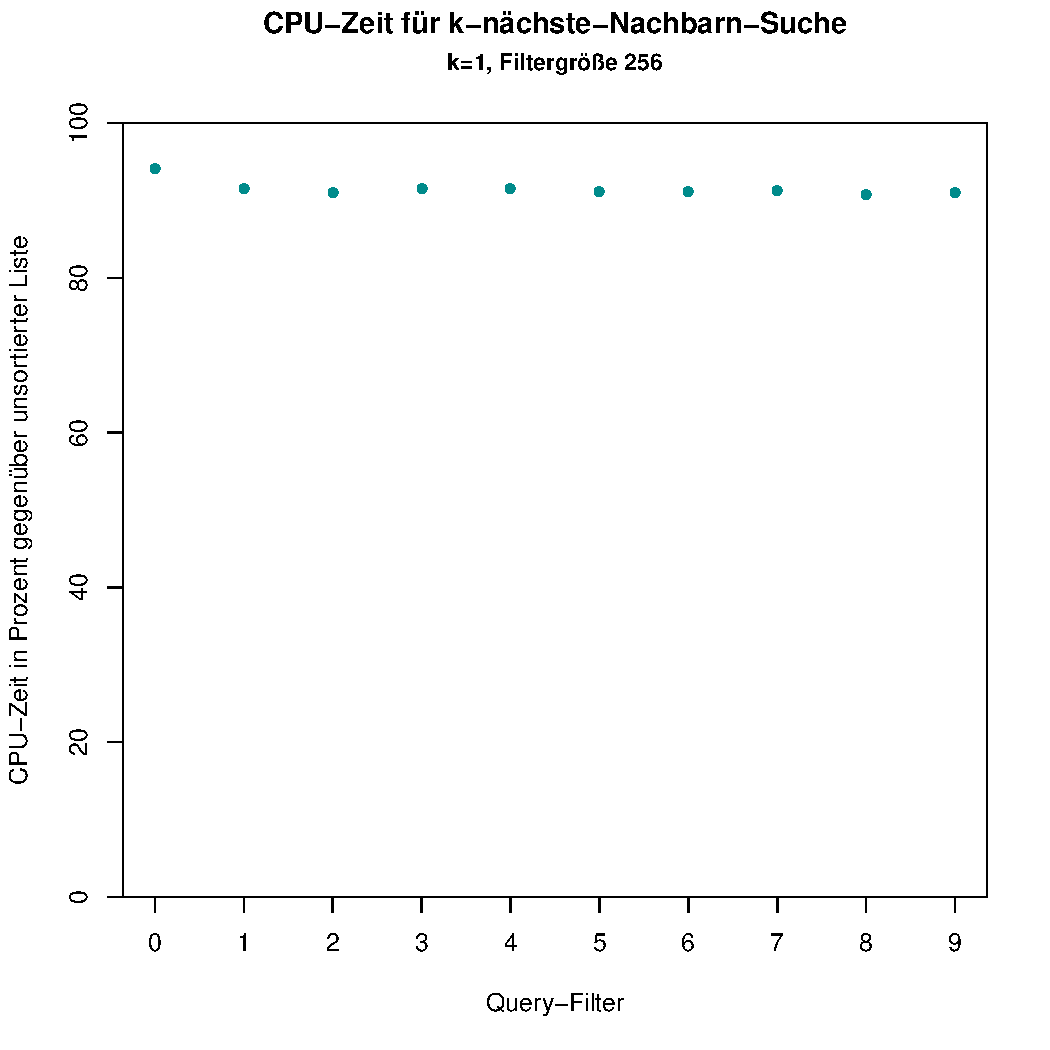
\includegraphics[width=0.48\linewidth]{pictures/percent_time_nn_256.pdf}}
	\hspace{0.01\textwidth}
	\subfloat[]{
	\label{fig:zeitersparnis:2}
	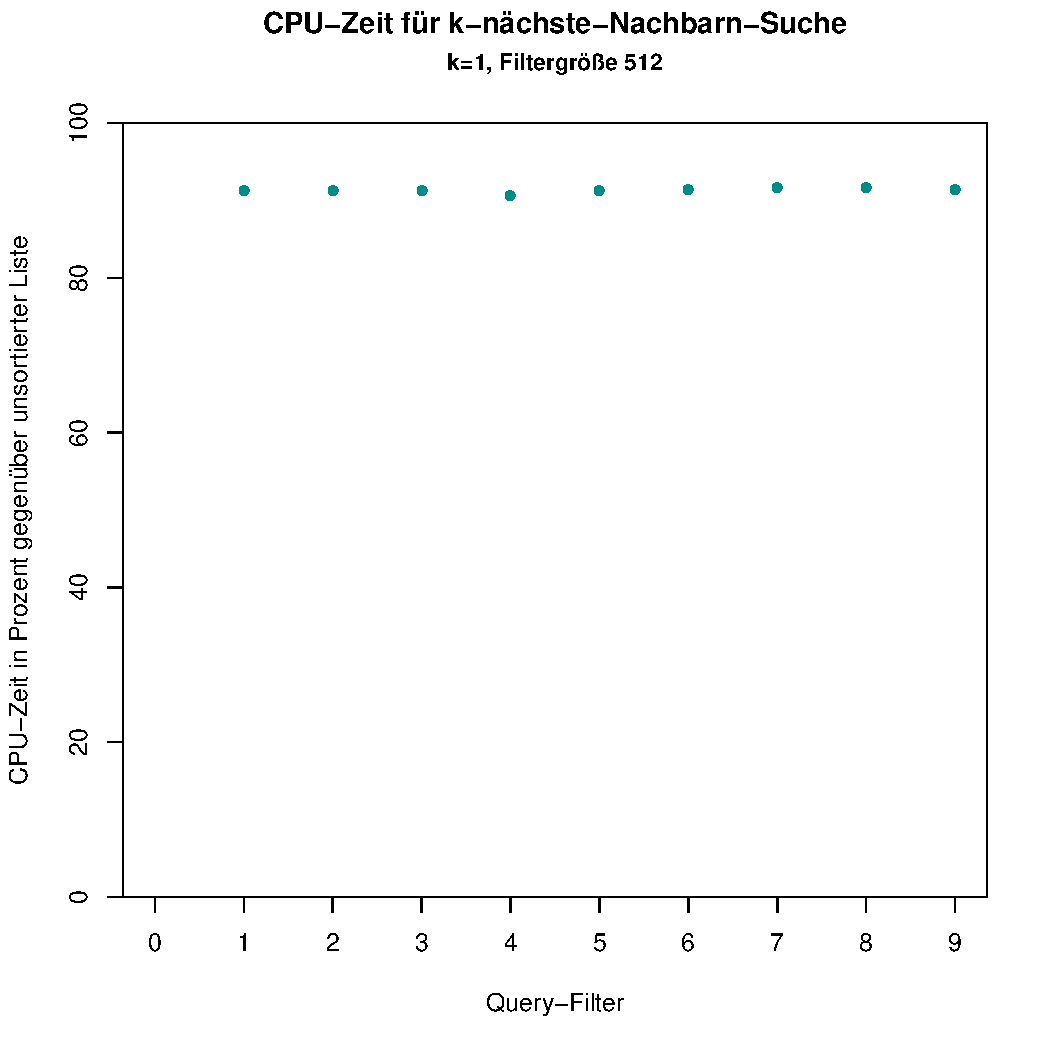
\includegraphics[width=0.48\linewidth]{percent_time_nn_512.pdf}}\\[0pt] % horizontal break
	\subfloat[]{
	\label{fig:zeitersparnis:3}
	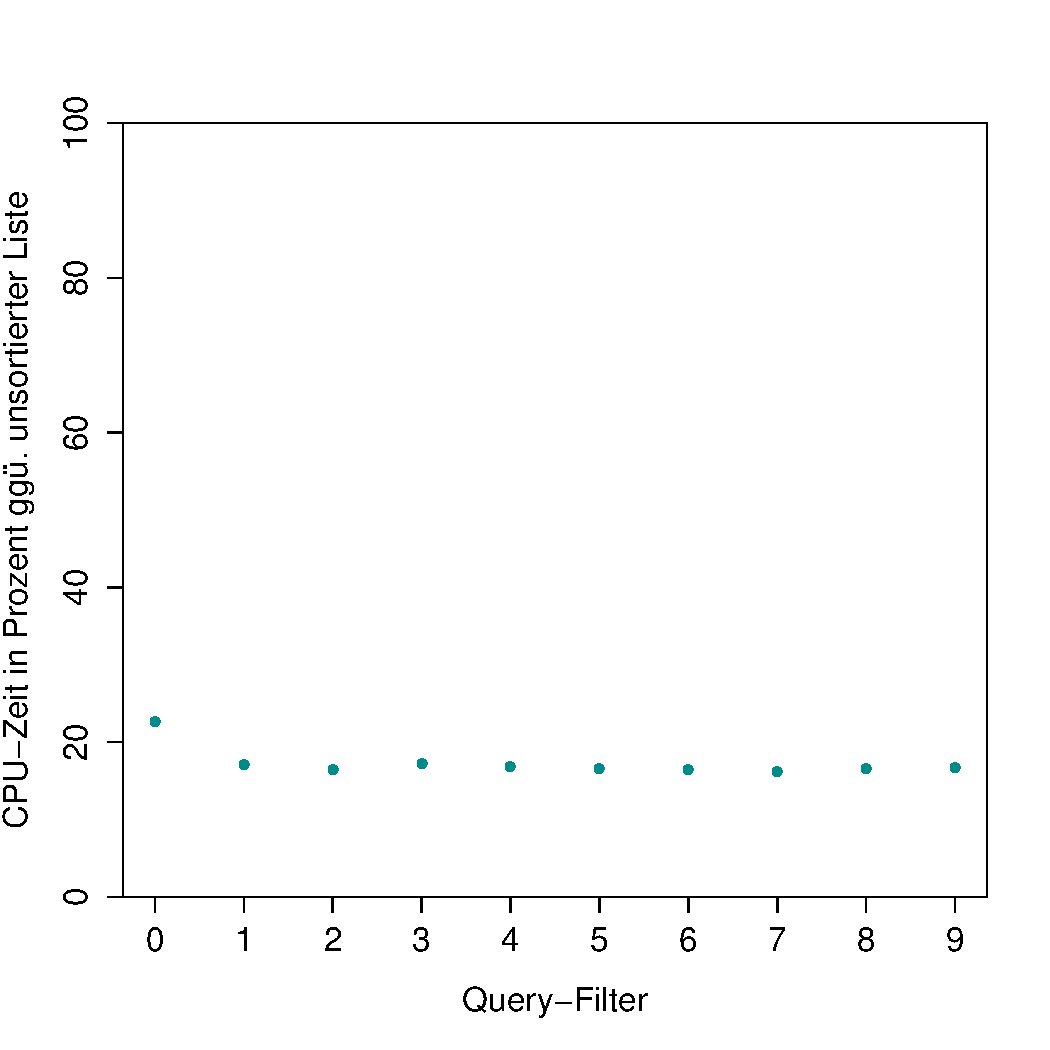
\includegraphics[width=0.48\linewidth]{pictures/percent_time_nn3_256.pdf}}
	\hspace{0.01\textwidth}
	\subfloat[]{
	\label{fig:zeitersparnis:4}
	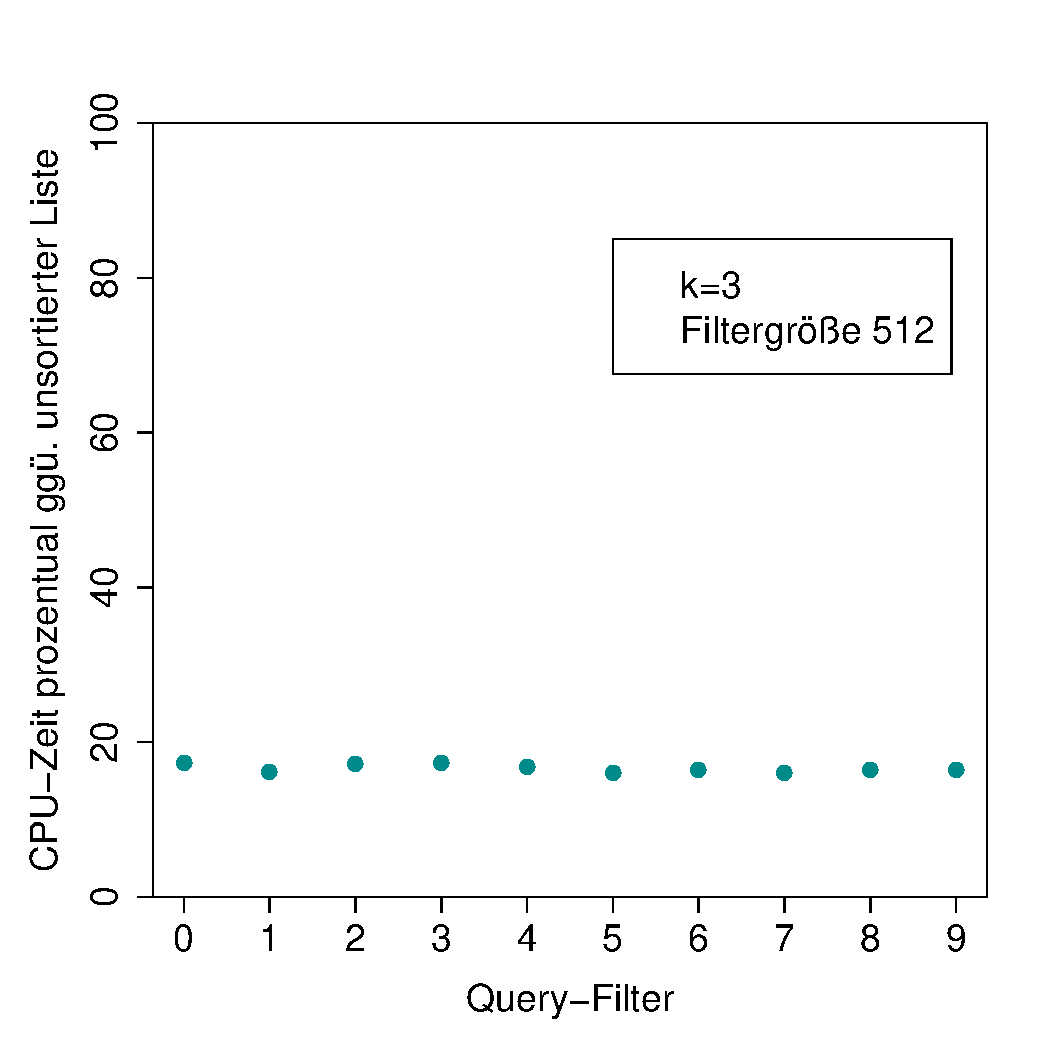
\includegraphics[width=0.48\linewidth]{pictures/percent_time_nn3_512.pdf}}
\end{figure}
Daran wird deutlich, dass die Zeitersparnis mit dem Parameter \textit{k} und der Filtergröße wächst, doch auch für $k=1$ wird bereits CPU-Zeit eingespart. Es ist zu erwarten, dass bei größeren BloomFilterTree-Objekten, höheren Anzahlen an Filtern und größeren Filtern die Zeitersparnis noch deutlich gesteigert werden kann: Beim hier verwendeten Versuchsaufbau werden in der Regel Bäume mit drei Ebenen aufgebaut, d.h. bei einer Punktanfrage wird auch bei bestehenden Teil- und Obermengenbeziehungen ein großer Teilbaum durchsucht bzw. ein großer Bereich der Blattebene traversiert. Bei größerer Höhe des Baums durch mehr eingefügte Filter kommen damit die Vorteile des entwickelten Verfahrens noch deutlicher zum Tragen. Wie in Abbildung \ref{fig:zeitersparnis} erkennbar, gilt dies ebenso für höhere Filtergrößen. Die CPU-Zeitersparnis zeigt sich bei Anfragen mit $k>1$ besonders deutlich. Auch hier ist zu erwarten, dass sich die Vorteile des entwickelten Verfahrens bei höheren Bäumen und Filteranzahlen sowie größeren Filtern noch deutlich stärker zeigen.

Wie in Abschnitt \ref{sec:b+bäume} dargestellt, ist die Komplexität der Suchoperation im B$^+$-Baum abhängig vom Parameter \textit{t}, d.h. dem Grad des Baumes. Die hier verwendeten Bloom\-Filter\-Tree-Objekte haben Grad 3, d.h. die maximale Ausfächerung beträgt 7. Dieser Parameter kann beim Anlegen eines BloomFilterTree-Objekts in der eigenen Implementierung frei gewählt werden. In der Praxis werden deutlich höhere Werte für \textit{t} verwendet, z.B. mit 10.000 Elementen pro Knoten beim Einsatz in Datenbank-Managementsystemen. Es ist daher davon auszugehen, dass die Anwendung für ein deutlich größeres Szenario prinzipiell gut geeignet wäre.  
\paragraph*{Speicherbedarf}
Der zusätzliche Speicherbedarf beim BloomFilterTree gegenüber einem Bloom-Filter-Vektor ergibt sich durch die Allokierung eines Vereinigungsfilters für jeden Knoten. Er ist somit abhängig von der Anzahl der Knoten im Baum. Mit dem verwendeten Versuchsaufbau liegt er um 32\% für den BloomFilter gegenüber einem Bloom-Filter-Vektor. Auch hier ließe sich durch eine geringere Knotenanzahl, d.h. BloomFilterTree-Objekte mit höherem Verzweigungsgrad, noch Speicherplatz einsparen.  
\paragraph*{Aufbaukosten}
Die Kosten für den Aufbau der Indexstruktur sind erwartungsgemäß ein Wermutstropfen. Auch wenn in der Praxis niedrigere Werte zu erwarten sind, da weniger als \textit{n} freie und "`gute"' IDs sortiert werden müssen, liegen die Aufbaukosten in $O(n\ast log(n))$. Das ist offensichtlich ein starker Zuwachs gegenüber einer unsortierten Liste, die sich z.B. durch ein Objekt vom Typ \texttt{std::vector} realisieren lässt. Andererseits kann davon ausgegangen werden, dass die Aufbaukosten in AMBIENCE deutlich seltener anfallen als z.B. in einem Verteilten System mit häufigem Ausscheiden und Hinzukommen von Knoten wie in den Abschnitten \ref{sec:bloom-netzwerk} und \ref{sec:bloom-index} beschrieben.
\paragraph*{Komplexität}
Auch bezüglich der Zeitkomplexität, d.h. der Abschätzung der notwendigen Berechnungsschritte unabhängig von der gewählten Plattform, zeigt das entwickelte Verfahren erfreuliche Ergebnisse. Die Anzahl der nötigen Vergleiche bei der \textit{k}-nächste-Nachbarn-Suche beträgt 24\% bzw. 32\% für $k=1$ bzw. $k=3$ beim BloomFilterTree gegenüber der unsortierten Liste. Auch hier ist zu erwarten, dass die Diskrepanz bei höheren Bäumen noch deutlicher zu Tage tritt, da bei der \textit{k}-nächste-Nachbarn-Suche nur der beste Pfad verfolgt wird. Bei höheren Bäumen werden somit mehr bzw. größere Teilbäume abgeschnitten und müssen nicht betrachtet werden.

Damit ist auch auf theoretischer Ebene der Nachweis erbracht, dass das entwickelte Verfahren zur Optimierung der \textit{k}-nächste-Nachbarn-Suche geeignet ist. Der BloomFilterTree lässt sich damit unabhängig von der verwendeten Maschine und der konkreten Implementierung zur Organisation von Bloom-Filtern in kontextzentrischen sozialen Netzen einsetzen. 